
%TODO: faltes d'ortografia, etc

\chapter{Optimitzacions}

En aquest apartat hem documentat les optimitzacions que hem anat aplicant al projecte incrementalment, es a dir, les hem aplicat una per una i hem mirat si realment teniem un guany de temps. 

Timing del codi original sobre la maquina de proves especificada al Apèndix B amb la qual s'han calculat els timings i speedups de les optimitzacions d'aquest apartat:
\begin{itemize}
\item{\textbf{Compilat amb el Makefile de l'apendix A, amb el que hem compilat totes les optimitzacions d'aquest apartat.}}
\item{Elapsed: 51.03s}
\end{itemize}


\section{Optimitzaci\'o 1: Loop roll}
\begin{itemize}
\item{Funció: motion.c/dist1}
\item{SpeedUp:1.07}
\item{Elapsed:47.45s}
\end{itemize}

A dist 1 hem detectat que hi havia un bucle desenrotllat. Hem decidit provar d'enrotllar-ho de nou i veure si el compilador aconseguia optimitzar més aquest unroll, i efectivament, amb el bucle enrotllat hi ha hagut un guany de temps, ja que el compilador genera un codi més eficient en el moment d'aplicar l'unroll. Per tant la feina d'aquest unroll la deixem al compilador.

\begin{lstlisting}
for (i = 0 ; i < 16 ; i++)
{
  if ((v = p2[i]  - p1[i])<0) v = -v;
}
\end{lstlisting}
 
\section{Optimitzaci\'o 2: Retallada d'iteracions innecessaries}
\begin{itemize}
\item{Funció: motion.c/dist1}
\item{SpeedUp: 1.21}
\item{Elapsed: 39.5s}
\end{itemize}

Analitzant una mica el codi de la funció dist1 a motion.c, hem vist que el que fa aquesta funció es acumular a la variable s distàncies absolutes i finalment retornar s. Peró hi ha un detall important en aquest codi: no volem calcular totalment s, sinó que el que en interessa es saber si $s>distlim$, un altre paràmetre de la funció.

Per tant, als bucles que acumulen distàncies absolutes a s, hem fet que sorti del bucle si s passa a ser major o igual que distlim. D'aquesta manera, ens estalviem gran quantitat de càlculs ja que dist1 es una funció que es crida gran quantitat de vegades als bucles de fullsearch.

\section{Optimitzaci\'o 3: Bithacks}
\begin{itemize}
\item{Funcio: motion.c/dist1}
\item{SpeedUp: -}
\item{Elapsed: 41.62s}
\end{itemize}

El bucle que hem desenrotllat a l'optimització 1 fa el següent a cada iteració: resta dos valors, els fa el valor absolut i els suma a s. El valor absolut el calcula amb un 

\begin{lstlisting}
if(v<0) v=-v 
\end{lstlisting}

per tant havíem pensat que fent bithacks ens podíem estalviar aquest salt. Hem aplicat el següent bithack:

\begin{lstlisting}
v = p2[i]  - p1[i];
v = (v ^ (v>>31)) - (v>>31);
\end{lstlisting}
 

D'entrada nomes l'hem aplicat al primer bucle de dist1 per veure si hi havia guany o no. Tot i això, el profiling d'aquest programa ha estat negatiu: es triga més amb aquest bithack que amb l'if. Es evident que el compilador amb els flags adequats d'optimització fa bastant bona feina amb algunes optimitzacions.
              

\section{Optimitzaci\'o 4: Loop splitting}
\begin{itemize}
\item{Funcio: motion.c/fullsearch}
\item{SpeedUp: 1.03}
\item {Elapsed: 38.91s}
\end{itemize}

El bucle:

\begin{lstlisting}
for(k=0; k<8*l; k++)
\end{lstlisting}

conté al final un if a on es decideix si mou j segons si el valor de k ha arribat a un cert valor. Aquest bucle es pot separar en 4 bucles a on a cadascun d'ells s'incrementa una variable (i,j i k en ordre), estalviant-nos l'if amb 3 condicions a cada iteració.

Com es pot veure, la millora no es massa notable, però suficient per deixar-la, a més aquesta modificació ens permetrà més endavant aplicar altres optimitzacions, com treure condicions a fora dels bucles.

\section{Optimitzaci\'o 5: Memoization}
\begin{itemize}
\item{Funció: motion.c/dist1}
\item{SpeedUp: -}
\item{Elapsed:41.21s} 
\end{itemize}

Analitzant els valors dels punters p1 i p2 a dist1, hem vist que aquests son valors entre 0 i 255  (típics valors de components de color y valors que caben a un unsigned char). Per tant vam pensar que potser fent memoization de les restes i valors absoluts d'aquests valors aconseguíem accelerar el proces a dist1. Vam fer servir una matriu de 255x255 amb totes les restes que s'inicialitzava al principi de l'execució. 

El profiling d'aquesta versió va donar temps molt semblants tot i que sempre pitjors que els de la versió sense memoization. Això ens indica que amb memoization es guanya poc temps, el qual es perd amb l'overhead inicial d'omplir aquesta matriu i amb el cost dels accessos a memòria de la matriu de memorització la qual s'accedeix de forma arbitraria i no s'aprofita gens la localitat espacial.

\section{Optimitzaci\'o 6: Especialitzaci\'o de dist1}
\begin{itemize}
\item{Funció: motion.c/dist1 $\Rightarrow$ dist1\_special}
\item{SpeedUp: 1.07}
\item{Elapsed: 36.42s}
\end{itemize}

Dist1 es crida des de fullsearch, la segona funció en el ranking de temps d'execució. Fullsearch crida a dist1 diverses vegades, inicialment amb paràmetres hx i hy =0, per tant hem decidit separar aquest cas de la dist1 genèrica per qualsevol hx i hy. D'aquesta manera en aquestes crides no s'haurà d'executar l'if tantes vegades.

\section{Optimitzaci\'o 7: Vectoritzaci\'o}
\begin{itemize}
\item{Funció: motion.c/dist1\_special , motion.c/dist1}
\item{SpeedUp: 2.04}
\item{Elapsed: 17.77s}
\end{itemize}

Com hem vist als dos intents anteriors d'optimitzar els calculs de dist1, no hem aconseguit un guany de temps important, per tant hem decidir atacar el problema amb la vectorització, ja que aquesta funció fa càlculs exactament de 16 bytes a cada iteració, el punter p2 sempre esta alineat, i l'increment dels punters lx sempre és múltiple de 16, per tant ens deixa en un bon escenari per aplicar vectorització.

El principal problema que vam veure es que el punter p1 no sempre és alineat, per tant hem separat dos casos. Quan p1 és alineat, hem aplicat una vectorització que fa servir l'intrinsic \texttt{\_mm\_sad\_epu8}, que fa exactament el que volem: difèrencies absolutes. Aquests resultats es guarden a un altre registre vectorial del que extraiem el resultat amb \texttt{\_mm\_extract\_epu16}.

\begin{lstlisting}
__m128i res;  
 
if(((unsigned int)p1 & 15) == 0)
{
  /* Dades alineades */
  __m128i *pr1,*pr2;

  for (j=0; j<h && s<distlim; j++,p1+=lx,p2+=lx)
  {   
    pr1 = (__m128i*) (((unsigned char *)p1));
    pr2 = (__m128i*) (((unsigned char *)p2));
		
    res=_mm_sad_epu8(*pr1, *pr2);
    s+=_mm_extract_epi16(res,0)+_mm_extract_epi16(res,4);
  }
}
else
{
  /* Dades no alineades */
  __m128i pr1,pr2;

  for (j=0; j<h && s<distlim; j++,p1+=lx,p2+=lx)
	{  
	  pr1 = _mm_loadu_si128( (__m128i*) p1);
	  pr2 = _mm_loadu_si128( (__m128i*) p2);
		
	  res=_mm_sad_epu8(pr1, pr2);
	  s+=_mm_extract_epi16(res,0)+_mm_extract_epi16(res,4);
	}  
}   
\end{lstlisting}

Com explicarem al punt següent, havíem pensat que potser seria bo que la part no alineada es fes amb threads per aplicar una mica totes les tècniques de les que disposem, però la idea no va resultar massa bona, ja que dist 1 es crida moltes vegades. Per aconseguir optimitzar una mica més, finalment vam fer la part no alineada amb vectorització no alineada, carregant les dades amb l'intrinsic de load unaligned, que tot i això va donar un speed up força bo respecte a la versió sense vectorització.

\section{Optimitzaci\'o 8: Threads}
\begin{itemize}
\item{Funció: motion.c/dist1\_special}
\item{SpeedUp: -}
\end{itemize}

Abans d'aplicar la vectorització tota "sencera", és a dir per posicions alineades i no alineades, teníem el cas que les no alineades seguien executant-se amb el bucle i utilitzant gprof, vam veure que aquesta part del codi, consumia gairebé un 80\% del temps de CPU. Per optimitzar aquest part, de seguida vàrem pensar en utilitzar els pthreads, ja que ens semblava un bon lloc i una bona manera d'aplicar una tècnica que encara no havíem fet servir fins ara. La idea era que cada thread executés un bucle i que es repartissin la feina entre ells. El codi quedava així:

\begin{lstlisting}
for (j=0; j<h/NUM_THREADS && s<distlim; j=j+NUM_THREADS){   
  for (t = 0; t < NUM_THREADS; t++){
  p1+=lx*(t+1);
  p2+=lx*(t+1);

  thread_data_array[t].distlim = distlim;
  thread_data_array[t].p1 = p1;
  thread_data_array[t].p2 = p2;

  rc = pthread_create(&threads[t],NULL,bucle_thread,
  (void *) &thread_data_array[t]);
}

for (t = 0; t < NUM_THREADS; t++){
  rc = pthread_join(threads[t],NULL);
  s = s + thread_data_array[t].s;
}		 	
\end{lstlisting}

La funció \texttt{blucle\_thread} és el bucle que fa els càlculs i tant els parametres d'entrada com de sortida están passats a través d'una estructura de dades creada i re-agrupada sota un array, un element per thread. La idea semblava que havia de donar bons results però el que no vam tenir en compte és en els càlculs reals que duu a terme \texttt{blucle\_thread}. En efecte, aquesta funció no fa masses iteracions i al contrari, és crida molts cops, per tant, l'overhead generat per crear i gestionar els threads era molt superior al temps guanyat. Això va provocar que descartéssim aquesta optimització per ineficient.

\section{Optimitzaci\'o 9: Code hoisting}
\begin{itemize}
\item{Funció: motion.c/fullsearch}
\item{SpeedUp: 1.04}
\item{Elapsed: 17.02s}
\end{itemize}

Un cop hem vectoritzat dist1, hem vist que tant dist1 com dist1\_special baixaven molt a la llista temps d'execució, i fullsearch es va quedar en primer lloc com a funció que triga més, per tant vam decidir centrar esforços en optimitzar fullsearch.

A fullsearch, recordant de les optimitzacions anteriors, tenim un bucle al que vam aplicar loop splitting per separar els casos a on s'incrementa//decrementa cada index (i,j). Això ens permet aplicar ara code hoisting i treure fora de l'if de dintre del bucle les condicions que tenen a veure amb l'index que no es modifica en aquell bucle. D'aquesta manera ja no cal ni entrar al bucle si la condició invariant no es compleix, directament modifiquem les variables que toca a fora del bucle, d'aquesta manera:

\begin{lstlisting}
if( i>=ilow && i<=ihigh){
  for (; k<(l<<2); k++,j++)
  {
    if (j>=jlow && j<=jhigh)
    {
      d = dist1_special(org+i+lx*j,blk,lx,0,0,h,dmin);
      mask=-(d<dmin);
      dmin=(dmin & ~mask) + (d&mask);
      imin = (imin & ~mask) + (i&mask);
      jmin = (jmin & ~mask) + (j&mask);
    }
  } 
}
else{
  j+=l<<1;
  k=l<<2;	
}	 	
\end{lstlisting}

\section{Optimitzaci\'o 10: Reducci\'o de constants a crides inicials}
\begin{itemize}
\item{Funció: motion.c/fullsearch}
\item{SpeedUp: 1.004 }
\item{Elapsed: 16.96s}
\end{itemize}

A fullsearch es fa una crida inicial a dist1 abans d'entrar al bucle de calcul, la qual es fa amb un valor constant. Aquest valor constant inicial es pot reduir, guanyant així una mica de temps i sense que es modifiqui la sortida del programa.

\section{Optimitzaci\'o 11: Bithacks a fullsearch}
\begin{itemize}
\item{Funció: motion.c/fullsearch}
\item{SpeedUp:  1.014}
\item{Elapsed:  16.72s}
\end{itemize}

Aquest bithack consisteix en substituir aquest codi:

\begin{lstlisting}
if (d<dmin)
{
  dmin = d;
  imin = i;
  jmin = j;
}
\end{lstlisting}

pel següent:

\begin{lstlisting}
mask=-(d<dmin);
dmin=(dmin & ~mask) + (d&mask);
imin = (imin & ~mask) + (i&mask);
jmin = (jmin & ~mask) + (j&mask);
\end{lstlisting}

D'aquesta manera ens estalviem els salts i tenim la mateixa sortida. A fullsearch hi ha diversos punts a on es pot aplicar, però per alguna raó només ens ha donat guany aplicant això a dos d'ells.

\section{Info general de les optimitzacions}

Finalment, adjuntem una gràfica comparativa dels temps obtinguts aplicant les diferents optimitzacions. Cal dir que son optimitzacions acumulatives, és a dir, que si una optimització ens ha aportat un millor temps, l'hem conservat. En el cas contrari, l'hem descartat. Al final hem aconseguit un \textbf{speedup de 3.05} corresponent a un \textbf{temps total d'execució de 16.72 s}. Tots aquests temps, han estat mesurats amb la màquina de proves del Apèndix B.


\begin{figure}[hbtp]
\begin{center}
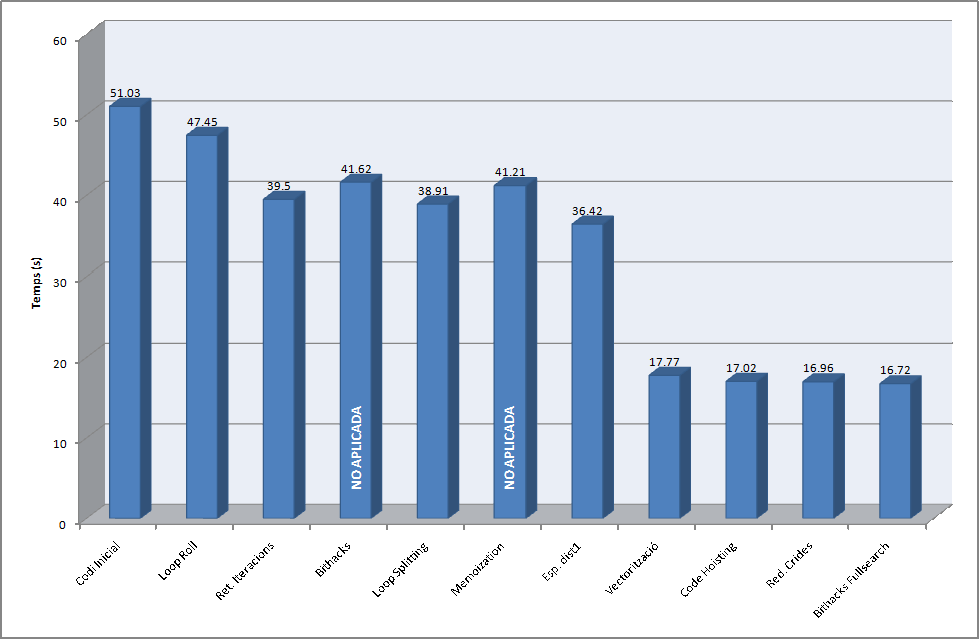
\includegraphics[scale=0.4]{img/image001.png}
\caption{Temps obtinguts amb les diferents optimitzacions}
\end{center}
\end{figure}
